This section introduces the elliptical PMCLP where there is no axis-parallel constraint, and the ellipses can be freely rotated. We refer to this problem as \sigla{MCER}{Maximal Covering by Ellipses with Rotation}. In comparison with MCE, this problem introduces a new variable that is responsible for determining the rotation angle of every ellipse, making MCER a more challenging problem.

\section{Definition}

An instance of the non-axis-parallel is defined exactly like the axis-parallel one on \autoref{chapter:ellipses}. It is given by a set of demand points $\Pp=\{p_1, \dots, p_n\}$, $p_j\in\R^2$; a list of weights $\Ww:=\{w_1, \dots, w_n\}$, with $w_j\in\R_{\ge0}$ being the weight of point $p_j$;
and $m$ ellipses given by their shape parameters $\Rr:=\{(a_1, b_1), \dots, (a_m, b_m)\}$, with $(a_j, b_j)\in\R_{>0}^2$ and $a_j>b_j$.
Additionally, to make the text more clear, we define a set of $m$ ellipses as $\E = \{E_1, \dots, E_m\}$, with $E_j : \R^2\times\R^2 \mapsto \R^2$ being a function that takes the center and angle of rotation where the $j$-th ellipse is located as input, and returns its coverage region as defined by \autoref{eq:rotated_ellipse_co}.
Lastly, an instance of MCER is defined as the tuple $(\Pp, \Ww, \Rr)$.

Given an instance of $MCER$, we define $Q:=(q_1, \dots, q_m) \in \R^{2m}$ to be the centers of each ellipse, $\Theta:=(\theta_1, \dots, \theta_m) \in [0, \pi)^m$ to be the angle of rotation of each ellipse and $E_i(q_i, \theta_i)$ to be the coverage region of ellipse $E_i$ with its center at point $q_i$ rotated by angle $\theta_i$, which is given by \autoref{eq:rotated_ellipse_co}. Therefore MCER is defined as the problem of determining $Q$ and $\Theta$ (placing and rotating each ellipse) to maximize the weight of points covered by the $m$ ellipses, which is given by

\begin{equation}\label{eq:optMCEn}
\max_{Q, \Theta}{w\left(\bigcup_{i=1}^{m} \Pp \cap E_i(q_i, \theta_i)\right)}.
\end{equation}
In addition to that, we define an equivalence relation between solutions of MCER. As likely expected, we say that two solutions are equivalent if the set of points covered by them is the same. In other words, two solutions of MCER $(Q, \Theta)$ and $(Q', \Theta')$ are said to be equivalent if, and only if 
$$\bigcup_{j=1}^m\Pp \cap E_j(q_j', \theta_j') = \bigcup_{j=1}^m\Pp \cap E_j(q_j, \theta_j).$$

Next, we introduce a proposition which says that given an optimal solution of MCER, it is possible to find another optimal solution with two points on the border of every ellipse that is already covering at least two points.

\begin{proposicao}\label{lema:mce_2b}
	Let $(Q^*, \Theta^*)$ be an optimal solution of an instance $(\Pp, \Ww, \Rr)$ of MCER. 
	Then, for any $E_j \in \E$ with $|\Pp \cap E_j(q_j^*, \theta_j^*)|\ge2$, 
	an equivalent solution $(Q', \Theta^*)$ exists, such that $|\Pp \cap \partial E_j(q_j', \theta_j^*)|\ge 2$.
\end{proposicao}

\begin{proof}
	First, the angle of rotation can be ignored as it does not change.
	
	Let $A=\Pp \cap E_j(q_j^*, \theta_j)$ be the set of points covered by the $j$-th ellipse and $X=\cap_{p \in A}E_j(p, \theta_j)$ be the region of intersection of ellipses centered at each point from $A$.

	As it was shown on \autoref{chapter:ellipses}, $X$ is a region that is limited by arcs of ellipses. As this region is the non-empty intersection of more than one ellipse, there are at least two of these arcs that encounter at one point, creating a vertex. Selecting any of these vertices as $q_j'$ will make $|\Pp \cap \partial E_j(q_j', \theta_j)| \ge 2$.
	
\end{proof}

What \autoref{lema:mce_2b} is saying is that any optimal solution for MCER can be transformed into another optimal solution where every ellipse covers the same set of points and those which cover more than one point has two points on their border. Also, this equivalent optimal solution can be always achieved by just translating the ellipses. An example is shown on \autoref{fig:ellipse-2-points} for one ellipse.

A lot of the ideas developed in this chapter are based on fixing two points on the border of an ellipse, which is why \autoref{def:feasible_angle} introduces a new notation for angles that an ellipse rotated by it can be translated into a center, such that it contains two fixed points. 

\begin{figure}
	\centering
	\caption{An optimal solution before and after applying \autoref{lema:mce_2b}.}
	\includegraphics{tex/figures/scripts/ellipse-2-points}
	\fautor
	\label{fig:ellipse-2-points}
\end{figure}

\begin{definicao}\label{def:feasible_angle}
	Let $E$ be the coverage region of an ellipse and $u, v \in \R^2$. An angle $\theta \in [0, \pi)$ is said to be $(E, u, v)$-feasible if there is $q \in \R^2$ such that $\{u, v\} \subset \partial E(q, \theta)$.
	In addition to that, given an instance of MCER, we refer to the set of $(E_j, u, v)$-feasible angles as 
	
	\begin{equation}
	\Phi_j(u, v) := \{\theta \in [0, \pi] : \theta \textnormal{ is a } (E_j,u,v)\textnormal{-feasible angle}\}.
	\end{equation}
\end{definicao}

In \autoref{fig:feasible-angle} two examples for \autoref{def:feasible_angle} are shown. The example with a solid contour shows an ellipse rotated by $\pi/4$ with two points on its border, making $\pi/4$ a $(E, u, v)$-feasible angle.
The other example, with a dashed contour, presents a case where an ellipse rotated by $\pi/2$ is not able to have the two points on its border, no matter where it is placed; because of that, $\pi/2$ is said to be a not $(E, u, v)$-feasible angle.

\begin{figure}[H]
	\centering
	\caption{A $(E, u, v)$-feasible angle and a not $(E, u, v)$-feasible angle.}
	\includegraphics[scale=.8]{tex/figures/scripts/feasible-angle}
	\fautor
	\label{fig:feasible-angle}
\end{figure}

In \autoref{chapter:definitions}, it was stated that the line that has the most distant intersection points with an ellipse is the one that passes through the origin, given that the linear parameter is fixed. It also says that the function $D$ given by \autoref{eq:dist_line_ellipse}, which represents the distance between the intersection points (it is negative when there is no intersection), attains every value less than its maximum.
This result provides a direct way to check if a certain angle $\theta\in[0, \pi]$ is feasible or not: rotate the points by $-\theta$ and check if $D(m, 0)$ is $\ge d$ with $m$ being the angular coefficient of the line that passes through the two points, and $d$ being the distance between them.

Furthermore, in \autoref{eq:dist_line_ellipse}, it can also be observed that $D(m, 0)^2$ is a parabola, which means that the set $\{m\in\R: D(m, 0)^2 \ge d^2\}$ is the union of at most two intervals. From there, given an instance of MCER, it is possible to arrive at the conclusion that a set of feasible angles for an ellipse and two points can be written as

\begin{equation}\label{eq:phi_j}
\Phi_j(u,v) = [\theta_1, \theta_2] \cup [\theta_3, \theta_4], 
\end{equation}
where $\theta_i$, $i=1\dots 4$, can be obtained from the solutions of $D(m, 0)^2=d$ and the extreme points $\{0, \pi, \pi/2\}$.
As a final remark, the angle which makes the two points form a vertical line deserves special treatment as its line cannot be represented by the equation $y=mx$.

\begin{lema}\label{lema:3pnts}
Let $(Q^*, \Theta^*)$ be an optimal solution of an instance $(\Pp, \Ww, \Rr)$ of MCER. Then, for any $E_j \in \E$, such that $|\Pp \cap E_j(q_j^*, \theta_j^*)|>2$, the following statements are equivalent:
	
	\begin{enumerate}[label=(\alph*)]
		\item $|\Pp\cap \partial E_j(q'_j, \theta'_j)| < 3$, for any equivalent solution $(Q', \Theta')$, \label{lema:3pnts_a}
		
		\item There is $\{u, v\}\subset\Pp \cap E_j(q_j^*, \theta_j^*)$, such that for any $\theta'\in\Phi_j(u,v)$, there is $q\in\R^2$, such that $\{u, v\} \subset \partial E_j(q, \theta)$ and $\Pp \cap E_j(q^*_j, \theta^*_j) = \Pp \cap E_j(q, \theta)$.\label{lema:3pnts_b}
	\end{enumerate}
\end{lema}

\begin{proof}
	To make the text more clear, let $A=\Pp\cap E_j(q^*_j, \theta^*_j)$.
	
	$\Rightarrow$
	
	According to \autoref{lema:mce_2b}, there exists $\{u, v\} \subset \Pp$, such that an equivalent optimal solution $(Q', \Theta^*)$ exists with $u, v$ on the border of $E_j(q_j', \theta_j^*)$. Therefore, $\theta_j^*\in\Phi_j(u,v)$.
	
	Suppose that $|\Phi_j(u,v)|>1$ 
	
	We are going to prove that if \autoref{lema:3pnts}\ref{lema:3pnts_a} is false, then \autoref{lema:3pnts}\ref{lema:3pnts_b} is true; and if \autoref{lema:3pnts}\ref{lema:3pnts_b} is false, then \autoref{lema:3pnts}\ref{lema:3pnts_a} is true.
	
	Before that, let us define $\Phi_j'$ as the open interval version of $\Phi_j$ as $\Phi_j'(u,v) = (\theta_1, \theta_2)\cup(\theta_3, \theta_4)$.
	
	Suppose that \autoref{lema:3pnts}\ref{lema:3pnts_a} is false.  

	
	For any $\theta\in\Phi_j'(u,v)$, we have get an 
\end{proof}

The first case of \autoref{lema:3pnts} is saying that there is another optimal solution which has $E_j$ covering the same set of points, but with three points on its border. 

The second case of \autoref{lema:3pnts} says that after fixing a pair of points on the border of $E_j$ maintaining the covered set, for any angle that allows the two points to stay on the border of $E_j$, there is a center that maintains the covered set the same.

On \autoref{fig:lema-3-points} both cases of \autoref{lema:3pnts} are shown. There, it can be seen that for the second case, it does not matter which feasible angle by which the ellipse is rotated, the third point will always be inside the coverage area. Also, an example of the first case is shown where there are three points lie exactly on the border of the ellipse.

\begin{figure}
	\centering
	\caption{An example of \autoref{lema:3pnts}.}
	\includegraphics[scale=.8]{tex/figures/scripts/lema-3-points}
	\fautor
	\label{fig:lema-3-points}
\end{figure}

The idea to prove \autoref{lema:3pnts} is that after fixing $u, v$ on the border of $E_j$, which is possible by \autoref{lema:mce_2b}, the movement of rotation and translation while keeping $u, v$ on the border is continuous. Because of that, the negation of case two implies case one and vice versa.


If we define an equivalence relation between optimal solutions as: $S_1$ is equivalent to $S_2$ if they both cover the same set of points, we can use \autoref{lema:3pnts} and \autoref{lema:mce_2b} to identify the equivalence classes. Let $S$ be any optimal solution, in $[S]$ (its equivalence class) there is another solution where any ellipse $E_j \in \E$ falls in at least one of the cases below:
\begin{itemize}
	\item $E_j$ covers only one point.
	\item $E_j$ covers more than one point with $u$ and $v$ being on the border of $E_j$. Note that there could be infinitely many of solutions like that, however, \autoref{lema:3pnts} guarantees that any $(E_j, u, v)$-feasible angle yields an equivalent optimal solution.
	\item $E_j$ covers more than two points with three of them on its border.
\end{itemize}

The following two sections will treat the second and third cases (the first case is trivial). Going through every possibility of an ellipse falling in any of the three cases guarantees that an optimal solution is found.

\section{Ellipse by two points}

Let $E$ be an ellipse with shape parameters $(a, b)\in \R^2_{>0}$ and $u, v\in \R^2$, one wants to find a $(E, u, v)$-feasible angle $\theta\in[0,\pi]$ and every center $q\in\R^2$ such that $\{u, v\} \subset \tilde{E}(q, \theta)$.

For a fixed angle, finding every center such that two points are on the border of the ellipse is done on \autoref{chapter:ellipses_intersection}, from there we know that there could be at most $2$ of such centers. The only thing left to be done is finding a feasible angle. It turns out that the angle that makes the major-axis of the ellipse to be aligned with the line that passes through $u$ and $v$ will be a feasible angle if, and only if the set of feasible angles is not empty. This can be seen geometrically as other angles achieve a lesser maximum distance between the two points on the border.

\section{Ellipse by three points}


